\en{\fr{Soit $ABC$ un triangle tel que $\angle CAB=90^{\circ}$. Soient $D,E$ des points sur $AC$ et $AB$, respectivement, tels que $BCDE$ est un quadrilatère inscrit. Soient $\Omega_1,\Omega_2$ les cercles qui passent par $A$ et qui sont centrés en $E,D$, respectivement. Soit $P$ le deuxième point d'intersection de $\Omega_1$ et $\Omega_2$. Montrer que la droite $AP$ coupe $BC$ en deux.}
\en{
Let $ABC$ be a triangle with $\angle CAB = 90^{\circ}$. Let $D,E$ be points on $AC,AB$ respectively such that $BCDE$ is cyclic. Let $\Omega_1,\Omega_2$ be the circles through $A$ with centres $E,D$ respectively. Denote by $P$ the second intersection of $\Omega_1$ and $\Omega_2$. Prove that the line $AP$ bisects the side $BC$.
}

\de{
Sei $ABC$ ein Dreieck mit $\angle CAB = 90^{\circ}$. Seien $D,E$ zwei Punkte jeweils auf $AC, AB$ sodass $BCDE$ ein Sehnenviereck ist. Seien $\Omega_1,\Omega_2$ die Kreise durch $A$ mit jeweiligen Mittelpunkten $E,D$. Sei $P$ der zweite Schnittpunkt von $\Omega_1$ und $\Omega_2$. Beweise, dass die gerade $AP$ die Strecke $BC$ halbiert.
}

\begin{center}
	%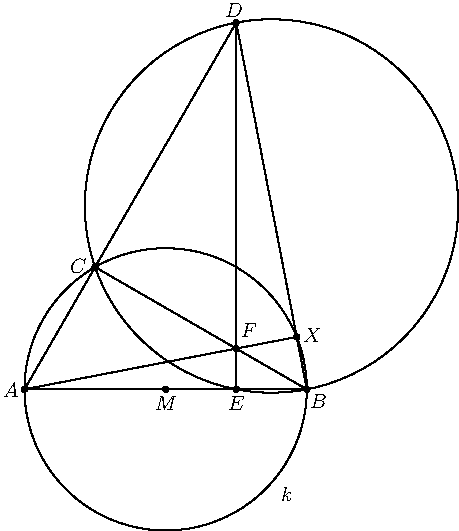
\includegraphics{2022/Final Round/Master Solution/fig-f1.pdf}
\end{center}
\vspace{0.8cm}
\textbf{Answer:} $BX/XD =1/6$.
\newpage
\textbf{First solution (Florian):} 
Let $s=AM$.
According to the conditions in the exercise we get:
\[
s=AM=MB=\frac{1}{2}AB=AC=\frac{1}{2}CD=\frac{1}{3}AD
\]
Using the power of the point $A$ with respect to the circle $EBDC$
\[
AE=\frac{AC\cdot AD}{AB}=\frac{s\cdot 3s}{2s}=\frac{3s}{2}
\]
and therefore
\[
EB=AB-AE=\frac{s}{2}.
\] 
Since $F$ is an inner point of the triangle $ABD$, applying Ceva's theorem gives
\[
1=\frac{BX}{XD}\cdot \frac{DC}{CA}\cdot \frac{AE}{EB}=\frac{BX}{XD}\cdot \frac{2s}{s} \ \frac{3s/2}{s/2} =6\cdot \frac{BX}{XD}\quad
\Longrightarrow\quad \frac{BX}{XD} =\frac{1}{6}.
\]

\textbf{Second solution:}
Using Thales' theorem over the circles $k$ and $EBCD$ gives
  \[
 90^{\circ}=\angle ACB=\angle DCB=\angle DEB.
 \]
Therefore, $DE$ and $BC$ are altitudes of the triangle $ABD$. Thus, $F$ is the orthocenter of $ABD$. It follows that $EBDC$, $AEXD$ and $ABXC$ are cyclic quadrilaterals (in particular $X \in k$).

By power of the points $A,B,D$ with respect to the circles $EBDC$, $AEXD$, $ABXC$ (individually) we get
   \[ AE\cdot AB=AC\cdot AD,\]
   \[ BE\cdot BA=BX\cdot BD,\]
   \[ DX\cdot DB=DC\cdot DA.\]
Up to this point, we have not used any of the conditions about the lengths. Like in the first solution, we define $s=AM$ and get
 \[
s=AM=MB=\frac{1}{2}AB=AC=\frac{1}{2}CD=\frac{1}{3}AD.
 \]
Finally
   \[
       \frac{BX}{XD}=\frac{BX\cdot BD}{DX\cdot DB}=\frac{BE\cdot BA}{DC\cdot DA}=\frac{AB^2-AE\cdot AB}{DC\cdot DA}=\frac{AB^2-AC\cdot AD}{DC\cdot DA}=\frac{(2s)^2-s\cdot 3s}{2s\cdot 3s}=\frac{1}{6}.
   \]

\newpage

 \textbf{Marking scheme:}
 
\textbf{Solution 1}
 \begin{enumerate}
 	\item Stating $\frac{BX}{XD} =\frac{1}{6}$ \dotfill (1 point)
 	\item Proving $EB=\frac{s}{2}$ or $AE=\frac{3s}{2}$, for $s=AM$ or any distance such as  $MB$, $\frac{1}{2}AB$, $AC$, $\frac{1}{2}CD$, $\frac{1}{3}AD$ \dotfill (3 points)
 	\item Using Ceva's theorem on point $F$ with respect to triangle $ABD$ \dotfill (2 points)
 	\item Conclude \dotfill (1 point)
 \end{enumerate}
\emph{Note: It is not necessary to mention right angles, altitudes or the fact that $X$ lies on $k$.}

\textbf{Solution 2}
	
\begin{enumerate}
		\item Stating $\frac{BX}{XD} =\frac{1}{6}$ \dotfill (1 point)
		\item Proving $AB \perp DE$ and $AD \perp BC$ \dotfill (1 point)
		\item Concluding that $F$ is the orthocenter of $ABD$ \dotfill (1 point)
		\item Proving that $AEXD$ and $ABXC$ are cyclic \dotfill (1 point)
		\item Proving the following 3 identities \dotfill (2 points)
   		\[ AE\cdot AB=AC\cdot AD\]
		\[ BE\cdot BA=BX\cdot BD\]
		\[ DX\cdot DB=DC\cdot DA\]
		Proving 1 of the last two identities is worth \dotfill (1 point)
		\item Conclude \dotfill (1 point)
	\end{enumerate}
	\emph{Note: To prove (b), (c), (d) and (e) it is not required to use any of the given conditions about the lengths. The fact $X \in k$ must be proven explicitly. If it is not the case, then \textbf{at most 4 points} are awarded.}
}